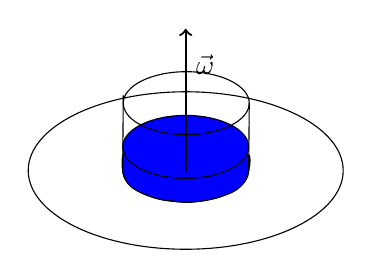
\begin{tikzpicture}

\draw  (0.5,-1) node (v1) {} ellipse (2 and 1);
\draw  (v1) ellipse (0.8 and 0.4);
\draw  [fill=blue]plot[smooth, tension=.7] coordinates {(-0.3,-0.8) (-0.3,-1) (-0.2,-1.2) (0.0788,-1.3376) (0.3191,-1.386) (0.6,-1.4) (0.9556,-1.3272) (1.2,-1.2) (1.3,-1) (1.3,-0.8) (1.1635,-0.9084) (0.9539,-1.0102) (0.6409,-1.0865) (0.3037,-1.0817) (0,-1) (-0.1881,-0.8594) (-0.29,-0.7)};

\draw [fill=blue] (0.5,-0.7) ellipse (0.8 and 0.4);
\draw []  (0.5069,-0.1448) ellipse (0.8 and 0.4);
\draw (-0.2931,-0.0448) -- (-0.3004,-1.0114) node (v3) {};
\draw (1.3069,-0.1448) -- (1.3,-1) node (v2) {};
\draw [->, thick](v1.center) -- (0.5,0.8)node[near end, right]{$\vec{\omega}$};

\end{tikzpicture}